
%\item Brief summary of results
The full results are listed in Appendix~\ref{sec:Appendix}. % Summarize results


%\item Interpretation of results
These results do not present clear evidence that the Reggio Approach is an effective early childhood program. However, there are several considerations about the evaluation context and the data. We consider the possibility that it is possible that as the programs evolved, they shared more features. In order to understand the trajectory of the programs, we wrote a survey to structure interviews with key individuals in the different school systems of Reggio Emilia, Parma, and Padova (see Appendix~\ref{sec:survey} for a full copy of the survey). In order to elicit a comparison with the Reggio Approach, we asked if the schools had aspects that are also present in the Reggio Approach schools. These key features that make up the Reggio Approach were collected from published materials as well as confirmed by staff of the Reggio Approach. 

We present the similarities and differences between the different programs in Figures~\ref{fig:agg-admin} and~\ref{fig:agg-ped}. Using results from the structured interviews, we compute the number of administrative and pedagogical components that each program shares with the Reggio Approach by school type, city, and year. We examine 14 administrative components and 12 pedagogical components. Over time, many of the programs other than the state programs, adopt more features present in the Reggio Approach. This is especially true of the Parma municipal program.

\begin{figure}[H]
\begin{center}
\begin{subfigure}[b]{0.5\textwidth}
	\caption{Number of Administrative Characteristics in Common with the Reggio Approach}\label{fig:agg-admin}
	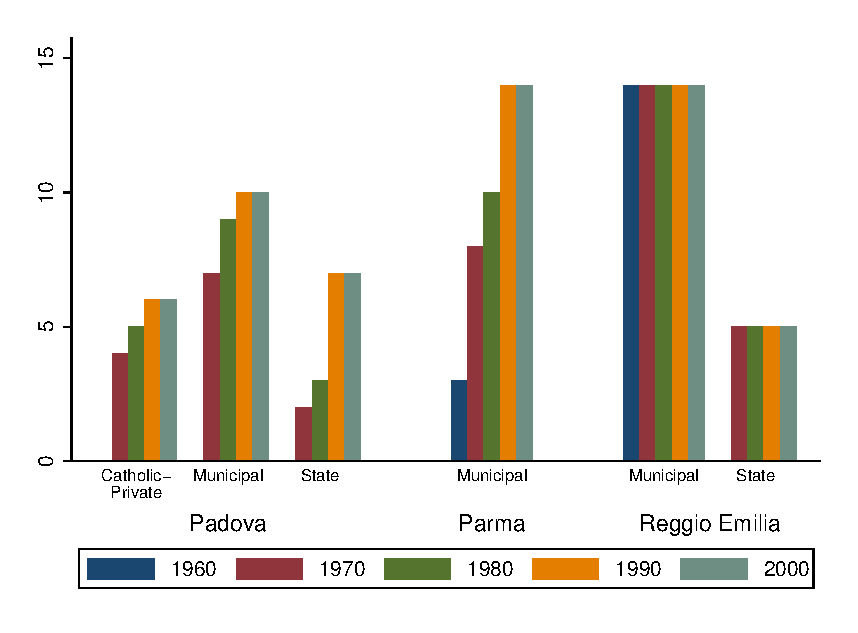
\includegraphics[width=0.8\textwidth]{../../output/aggregateAdministrative.eps}
\end{subfigure}%
~
\begin{subfigure}[b]{0.5\textwidth}
	\caption{Number of Pedagogical Characteristics in Common with the Reggio Approach}\label{fig:agg-ped}
	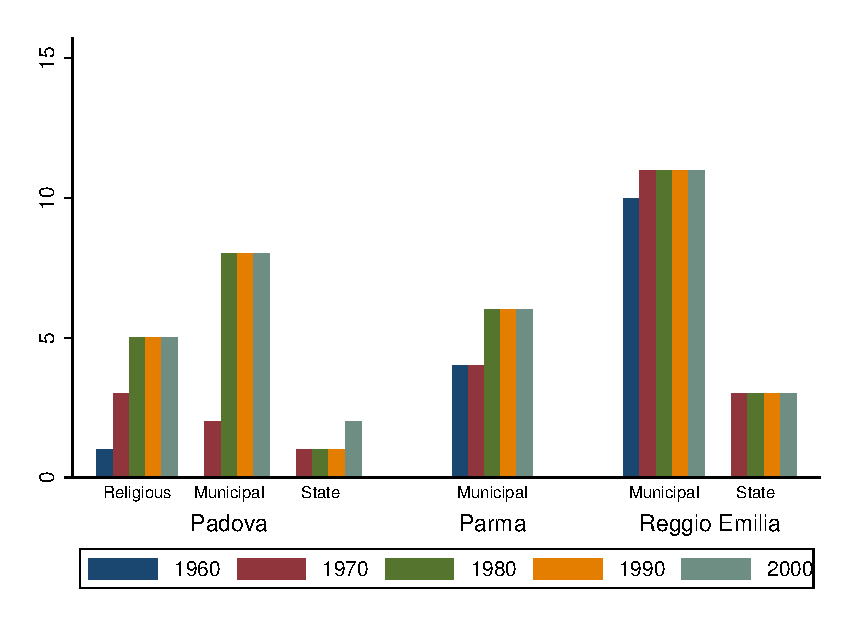
\includegraphics[width=0.8\textwidth]{../../output/aggregatePedagogical.eps}
\end{subfigure}%
\end{center}
\raggedright \footnotesize Note: These graphs show the number of administrative and pedagogical components that each program has in common with the Reggio Approach. We consider 14 administrative components and 12 pedagogical components. 
\end{figure}

%\item Expand discussion of survey highlighting specific questions that presented interesting results
In addition to this historical context, we expand on shortcomings in the data that make more precise analysis difficult.

\begin{enumerate}
	\item Selection issues
	\begin{enumerate}
		\item With more background variables for the adult cohorts, matching might be more successful
		\item With more accurate information on the distance to the nearest school, an instrumental variable approach might work
		\item Complete information on tuition costs would help understand the selection
		\item Discuss differences in eligibility requirements between cities and schools and how that might have contributed to differential selection
	\end{enumerate}
	\item Data issues
\end{enumerate}


